\begin{figure}[h]
    \centering
    \begin{subfigure}[b]{0.496\textwidth}
        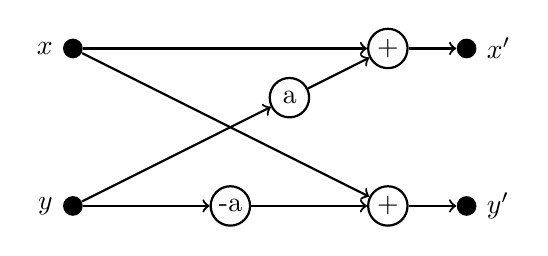
\begin{tikzpicture}[
                dot/.style = {circle, fill, inner sep = 0mm, minimum size = 2.5mm},
                op/.style = {draw, thick, circle, inner sep = 0mm, minimum size = 5mm},
                func/.style = {draw, thick, circle, inner sep = 1mm},
                arr/.style = {draw, thick, ->},
            ]
            \node (x) [dot, label=left:$x$] at (0,2){};
            \node (y) [dot, label=left:$y$] at (0,0){};
            \node (xp) [dot, label=right:$x'$] at (5,2){};
            \node (yp) [dot, label=right:$y'$] at (5,0){};

            \node (a1) [op] at (2.75, 1.375) {a};
            \node (a2) [op] at (2, 0) {-a};
            \node (p1) [op] at (4, 2) {+};
            \node (p2) [op] at (4, 0) {+};

            \path[arr] (x) -- (p1);
            \path[arr] (p1) -- (xp);
            \path[arr] (y) -- (a2);
            \path[arr] (a2) -- (p2);
            \path[arr] (p2) -- (yp);

            \path[arr] (x) -- (p2);

            \path[arr] (y) -- (a1);
            \path[arr] (a1) -- (p1);
        \end{tikzpicture}
        \caption{Butterfly structure.\label{fig:conva}}
    \end{subfigure}
    \begin{subfigure}[b]{0.496\textwidth}
        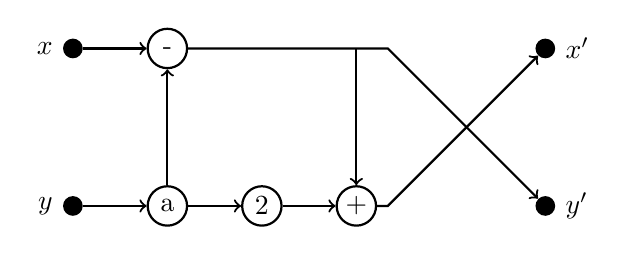
\begin{tikzpicture}[
                dot/.style = {circle, fill, inner sep = 0mm, minimum size = 2.5mm},
                op/.style = {draw, thick, circle, inner sep = 0mm, minimum size = 5mm},
                func/.style = {draw, thick, circle, inner sep = 1mm},
                arr/.style = {draw, thick, ->},
            ]
            \node (x) [dot, label=left:$x$] at (0,2){};
            \node (y) [dot, label=left:$y$] at (0,0){};
            \node (yp) [dot, label=right:$y'$] at (6,0){};
            \node (xp) [dot, label=right:$x'$] at (6,2){};

            \node (a) [op] at (1.2,0){a};
            \node (t) [op] at (2.4,0){2};
            \node (m) [op] at (1.2,2){-};
            \node (p) [op] at (3.6,0){+};

            \path[arr] (x) -- (m);
            \path[arr] (y) -- (a);
            \path[arr] (a) -- (m);
            \path[arr] (a) -- (t);
            \path[arr] (t) -- (p);
            \path[arr] (3.6,2) -- (p);

            \path[arr] (m) -- (4, 2) -- (yp);
            \path[arr] (p) -- (4, 0) -- (xp);
        \end{tikzpicture}
        \caption{Alternative lifting scheme.\label{fig:convb}}
    \end{subfigure}
    \caption{Datapaths for FFT convolution.\label{fig:conv}}
\end{figure}
